\Cref{fig:main} summarizes the main evidence. The reproduction anchor behaves as expected. At training size 450 and test size 600, the unconstrained edge ansatz reaches mean test accuracy $0.614\pm0.029$, while the $D_4$-equivariant edge ansatz reaches $0.688\pm0.036$ over five seeds. The generalization gap drops from $0.094$ to $0.023$. The unconstrained circuit has more parameters, but the additional freedom mostly appears as overfitting rather than useful test performance.

The subgroup sweep shows a more nuanced picture. Full $D_4$ is not beaten robustly by a partial group, so the conservative conclusion is not that less symmetry is better. Instead, $C_4$ tracks $D_4$ closely across data regimes: at 30 training examples, $C_4$ obtains $0.552$ test accuracy versus $0.531$ for $D_4$; at 120 examples, the two are essentially tied at $0.630$ and $0.629$; at 450 examples, $C_4$ and $D_4$ again match at $0.689$ and $0.688$. We interpret this as evidence that the useful inductive bias is not a single binary setting. Rotation-only equivariance can preserve nearly the same generalization behavior while relaxing part of the full constraint.

\begin{figure*}[t]
\centering
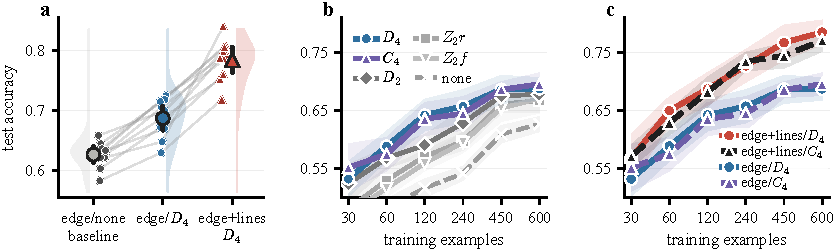
\includegraphics[width=\textwidth]{gfx/fig2_main_evidence}
\caption{Main empirical story. (a) Full $D_4$ equivariance improves test accuracy over no symmetry in the Meyer-style edge ansatz. (b) Across data regimes, $C_4$ closely follows $D_4$, while weaker or unconstrained sharing tends to lag. (c) The largest gain comes from keeping equivariance and adding task-aligned winning-line interactions. Error bars are 95\% confidence intervals over five seeds.}
\label{fig:main}
\end{figure*}

The strongest result is the oracle-inspired architecture. The Meyer-style edge/D4 model is around $0.69$ test accuracy in the robust sweep. Adding both winning-line interaction channels to the edge circuit increases performance to $0.795\pm0.016$ at 450 training examples and $0.805\pm0.019$ at 600 examples. The C4 version of the same architecture is also strong, reaching $0.778\pm0.013$ at 600 examples and $0.787\pm0.020$ at 750 examples. The improvement is therefore not obtained by breaking equivariance; it is obtained by using equivariance to tie a more task-aligned set of gates.

\begin{table}[t]
\centering
\caption{Key test-accuracy results used in the claims. Values are means with 95\% confidence intervals over five seeds.}
\label{tab:key}
\begin{tabular}{lccc}
\toprule
Model & Train & Params & Test acc.\\
\midrule
edge/none & 450 & 204 & $0.614\pm0.029$\\
edge/$D_4$ & 450 & 54 & $0.688\pm0.036$\\
edge/$C_4$ & 450 & 60 & $0.689\pm0.017$\\
random/$D_4$ & 450 & 54 & $0.572\pm0.026$\\
edge+both/$D_4$ & 450 & 90 & $0.795\pm0.016$\\
edge+both/$D_4$ & 600 & 90 & $0.805\pm0.019$\\
\bottomrule
\end{tabular}
\end{table}

\Cref{fig:controls} separates this effect from two simpler explanations. First, symmetry-aware sharing is not equivalent to arbitrary parameter reduction. At matched parameter counts, random tying is consistently worse: for $D_4$, symmetry-aware sharing gives $0.688$ while random sharing gives $0.572$; for $C_4$, the corresponding numbers are $0.689$ and $0.551$. Second, the oracle-inspired gain is not simply ``more parameters.'' Several models with similar or fewer parameters improve over the edge baseline, but the best result appears when the original edge interactions are combined with both winning-line channels. The parameter-count scatter shows the same point visually: the best circuit is not just farther to the right, it moves into a different accuracy region.

\begin{figure*}[t]
\centering
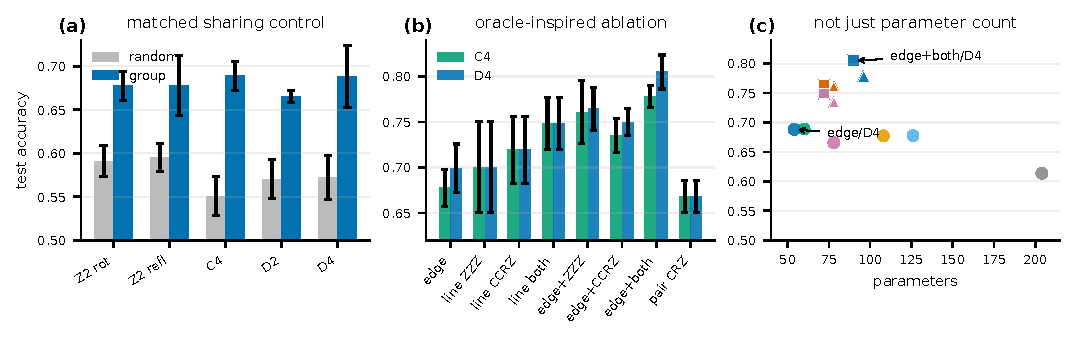
\includegraphics[width=\textwidth]{gfx/fig3_controls}
\caption{Controls and ablations. (a) Parameter-matched random sharing underperforms group-orbit sharing, so the benefit is not only fewer parameters. (b) Oracle-inspired ablations at 600 training examples show that the strongest model combines edge interactions with both winning-line channels. (c) Accuracy is not explained by parameter count alone; task-aligned equivariant geometry is the relevant change.}
\label{fig:controls}
\end{figure*}
